\subsection{k-reducibility}

\begin{frame}
    \frametitle{Rings}
    Rings play a key role in seperating a graph in two pieces with a common border.

    \begin{definition}
        A \emph{ring} of $n$ vertices $R_n$ in a planar graph $G$ is an induced cycle of $G$.
    \end{definition}

    \begin{figure}[!ht]
        \centering
        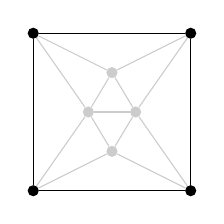
\begin{tikzpicture}
            \node[circle, fill, scale=0.015cm] (l1) at (-1, -1) { };
                \node[circle, fill, scale=0.015cm] (l2) at (-1, 1) { };
                \node[circle, fill, scale=0.015cm] (l3) at (1, 1) {};
                \node[circle, fill, scale=0.015cm] (l4) at (1, -1) {};
                \node[circle, fill, scale=0.015cm, opacity=0.2] (m1) at (0, 0.5) {};
                \node[circle, fill, scale=0.015cm, opacity=0.2] (m2) at (-0.3, 0) {};
                \node[circle, fill, scale=0.015cm, opacity=0.2] (m3) at (0.3, 0) {};
                \node[circle, fill, scale=0.015cm, opacity=0.2] (m4) at (0, -0.5) {};
    
                \draw (l1) -- (l2) -- (l3) -- (l4) -- (l1);
                \draw[opacity=0.2] (m1) -- (m2) -- (m4) -- (m3) -- (m1);
                \draw[opacity=0.2] (m2) -- (m3);
                \draw[opacity=0.2] (m1) -- (l2);
                \draw[opacity=0.2] (m1) -- (l3);
                \draw[opacity=0.2] (m2) -- (l1);
                \draw[opacity=0.2] (m2) -- (l2);
                \draw[opacity=0.2] (m3) -- (l3);
                \draw[opacity=0.2] (m3) -- (l4);
                \draw[opacity=0.2] (m4) -- (l1);
                \draw[opacity=0.2] (m4) -- (l4);
        \end{tikzpicture}
        \hspace{1cm}
        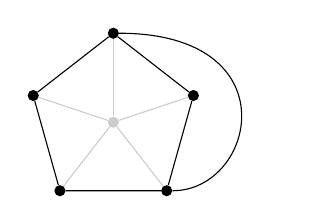
\begin{tikzpicture}[scale=1.13]
            \node[circle, fill, scale=0.015cm, opacity=0.2] (c) at (0, 0) {};
    
    
            \node[circle, fill, scale=0.015cm] (l1) at (0, 1) { };
            \node[circle, fill, scale=0.015cm] (l2) at (0.9, 0.30) { };
            \node[circle, fill, scale=0.015cm] (l3) at (0.6, -0.77) {};
            \node[circle, fill, scale=0.015cm] (l4) at (-0.6, -0.77) {};
            \node[circle, fill, scale=0.015cm] (l5) at (-0.9, 0.30) {};
    
            \draw[opacity=0.2] (c) -- (l1);
            \draw[opacity=0.2] (c) -- (l2);
            \draw[opacity=0.2] (c) -- (l3);
            \draw[opacity=0.2] (c) -- (l4);
            \draw[opacity=0.2] (c) -- (l5);
            \draw (l1) -- (l2) -- (l3) -- (l4) -- (l5) -- (l1);
            \draw (l1) .. controls +(2,0) and +(1,0) .. (l3);
        \end{tikzpicture}
        \caption{Valid ring (left). Invalid ring (right).}
        \label{fig:ring}
    \end{figure}
\end{frame}


\begin{frame}
    \frametitle{Ring colorings}

    \begin{definition}
        The set of all 4-colorings of a ring $R$ in a planar graph $G$ is given by $\Phi(R \subset G)$ or $\Phi(G)$ if $R$ is clear from the context.
    \end{definition}
    \begin{definition}
        The set of all ring colorings of $R_n$ is given by $\Phi(n) = \Phi(R_n)$.
    \end{definition}
\end{frame}


\begin{frame}
    \frametitle{Rings are reducible}

    A ring on its own is a reducible configuration.

    \begin{theorem}<1->
        \label{thm:ringsarered}
        The ring $R_n$ with $n\geq 4$ is reducible in every planar graph $G$.
    \end{theorem}
    \begin{proof}<2->
        Because $R_n$ is contained, the interior of $R_n$ is empty. Contract two non-neighboring vertices $v_1$ and $v_3$ to a new vertex $u$. We obtain the smaller graph $G'$. To reverse a coloring of $G'$, we give $v_1$ and $v_3$ the same color as $u$.
        We obtained a coloring for $G$.
    \end{proof}

    \uncover<2->{\begin{figure}[!h]
        \centering
        \begin{tikzpicture}[scale=0.7]
            \node (l1) at (-1, -1) { $a$ };
            \node (l2) at (-1, 1) { $b$ };
            \node (l3) at (1, 1) { $c$ };
            \node (l4) at (1, -1) { $b$ };
    
            \draw (l1) -- (l2) -- (l3) -- (l4) -- (l1);
            \node (impl) at (2.3, 0) { $\Longleftrightarrow$ };
            \draw[dotted, thick] (l2) -- (l4);
        \end{tikzpicture}
        \begin{tikzpicture}[scale=0.7]
            \node (l1) at (-1, -1) { $a$ };
            \node[opacity=0.2] (l2) at (-1, 1) { $b$ };
            \node (l3) at (1, 1) { $c$ };
            \node[opacity=0.2] (l4) at (1, -1) { $b$ };
            \node (c) at (0, 0) { $b$ };
    
            \draw (l1) -- (c) -- (l3);
            \draw[dotted, thick, opacity=0.2] (l2) -- (c) -- (l4);
        \end{tikzpicture}
    \end{figure}}
\end{frame}


\begin{frame}
    \frametitle{Ring configurations}
    \begin{definition}
        A planar graph $\confg = R_n + \core$ consisting of a ring $R_n$ and an interior $\core$ is called a \emph{ring configuration} on $R_n$. $\core$ is called the \emph{core} of $\confg$.
    \end{definition}

    \begin{figure}[!h]
        \centering
            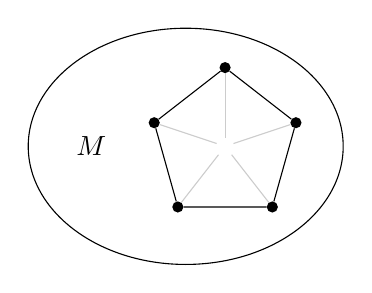
\begin{tikzpicture}
            \draw[fill=white] (-0.5, 0) ellipse (2cm and 1.5cm);
            %\draw[fill=lightgray, draw=black] (0,0) circle (1.25cm);
            %\draw[fill=white] (0,0) circle (0.75cm);
            \node at (-0.7, 0.9) {$\confg$};
            \node at (-1.7, 0) {$M$};
    
            \node[inner sep=1mm] (c) at (0, 0) {$\core$};
            \node[circle, fill, scale=0.015cm] (l1) at (0, 1) { };
            \node[circle, fill, scale=0.015cm] (l2) at (0.9, 0.30) { };
            \node[circle, fill, scale=0.015cm] (l3) at (0.6, -0.77) {};
            \node[circle, fill, scale=0.015cm] (l4) at (-0.6, -0.77) {};
            \node[circle, fill, scale=0.015cm] (l5) at (-0.9, 0.30) {};
    
            \draw[opacity=0.2] (c) -- (l1);
            \draw[opacity=0.2] (c) -- (l2);
            \draw[opacity=0.2] (c) -- (l3);
            \draw[opacity=0.2] (c) -- (l4);
            \draw[opacity=0.2] (c) -- (l5);
            \draw (l1) -- (l2) -- (l3) -- (l4) -- (l5) -- (l1);
        \end{tikzpicture}
    \end{figure}

    We have already shown reducibility if $\core = \varnothing$ (nothing)!
\end{frame}

\begin{frame}
    \frametitle{Finding common ring colorings}

    We split our graph into $M+R$ and $\core+R$. Now we try to find a common coloring on the ring $R$.
    \begin{figure}[!h]
        \centering
        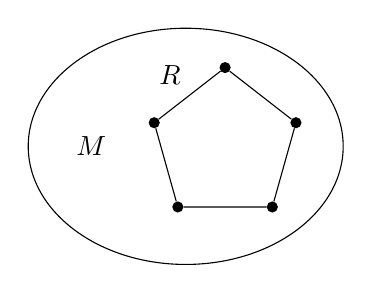
\begin{tikzpicture}
            \draw[fill=white] (-0.5, 0) ellipse (2cm and 1.5cm);
            \node at (-1.7, 0) {$M$};
            \node at (-0.7, 0.9) {$R$};
    
            \node[circle, fill, scale=0.015cm] (l1) at (0, 1) { };
            \node[circle, fill, scale=0.015cm] (l2) at (0.9, 0.30) { };
            \node[circle, fill, scale=0.015cm] (l3) at (0.6, -0.77) {};
            \node[circle, fill, scale=0.015cm] (l4) at (-0.6, -0.77) {};
            \node[circle, fill, scale=0.015cm] (l5) at (-0.9, 0.30) {};
    
            \draw (l1) -- (l2) -- (l3) -- (l4) -- (l5) -- (l1);
        \end{tikzpicture}
        \hspace{1cm}
        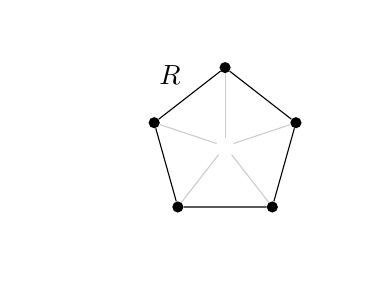
\begin{tikzpicture}
            \draw[fill=white, opacity=0] (-0.5, 0) ellipse (2cm and 1.5cm);
            %\draw[fill=lightgray, draw=black] (0,0) circle (1.25cm);
            %\draw[fill=white] (0,0) circle (0.75cm);
            \node at (-0.7, 0.9) {$R$};
    
            \node[inner sep=1mm] (c) at (0, 0) {$\core$};
            \node[circle, fill, scale=0.015cm] (l1) at (0, 1) { };
            \node[circle, fill, scale=0.015cm] (l2) at (0.9, 0.30) { };
            \node[circle, fill, scale=0.015cm] (l3) at (0.6, -0.77) {};
            \node[circle, fill, scale=0.015cm] (l4) at (-0.6, -0.77) {};
            \node[circle, fill, scale=0.015cm] (l5) at (-0.9, 0.30) {};
    
            \draw[opacity=0.2] (c) -- (l1);
            \draw[opacity=0.2] (c) -- (l2);
            \draw[opacity=0.2] (c) -- (l3);
            \draw[opacity=0.2] (c) -- (l4);
            \draw[opacity=0.2] (c) -- (l5);
            \draw (l1) -- (l2) -- (l3) -- (l4) -- (l5) -- (l1);
        \end{tikzpicture}
    \end{figure}

    Such a coloring might not always be guaranteed.
\end{frame}

\begin{frame}
    \frametitle{Reducers}

    We can add extra vertices on the other side of the ring. This restricts the possible colorings we can encounter.
    \begin{figure}[!h]
        \centering
        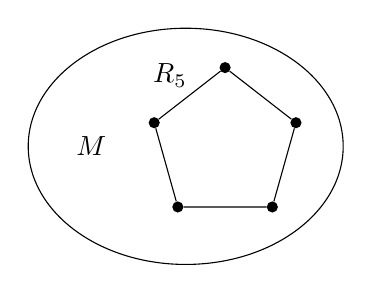
\begin{tikzpicture}
            \draw[fill=white] (-0.5, 0) ellipse (2cm and 1.5cm);
            \node at (-1.7, 0) {$M$};
            \node at (-0.7, 0.9) {$R_5$};
    
            \node[circle, fill, scale=0.015cm] (l1) at (0, 1) { };
            \node[circle, fill, scale=0.015cm] (l2) at (0.9, 0.30) { };
            \node[circle, fill, scale=0.015cm] (l3) at (0.6, -0.77) {};
            \node[circle, fill, scale=0.015cm] (l4) at (-0.6, -0.77) {};
            \node[circle, fill, scale=0.015cm] (l5) at (-0.9, 0.30) {};
    
            \draw (l1) -- (l2) -- (l3) -- (l4) -- (l5) -- (l1);
        \end{tikzpicture}
        \hspace{1cm}
        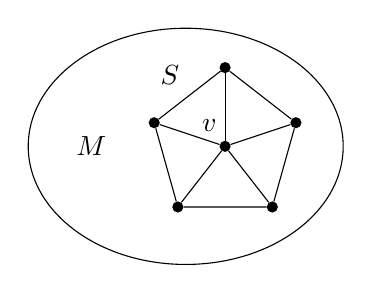
\begin{tikzpicture}
            \draw[fill=white] (-0.5, 0) ellipse (2cm and 1.5cm);
            \node at (-1.7, 0) {$M$};
            \node at (-0.7, 0.9) {$S$};
    
            \node (c) at (-0.2, 0.27) { $v$ };
            \node[circle, fill, scale=0.015cm] (c) at (0, 0) {};
            \node[circle, fill, scale=0.015cm] (l1) at (0, 1) { };
            \node[circle, fill, scale=0.015cm] (l2) at (0.9, 0.30) { };
            \node[circle, fill, scale=0.015cm] (l3) at (0.6, -0.77) {};
            \node[circle, fill, scale=0.015cm] (l4) at (-0.6, -0.77) {};
            \node[circle, fill, scale=0.015cm] (l5) at (-0.9, 0.30) {};
    
            \draw (c) -- (l1);
            \draw (c) -- (l2);
            \draw (c) -- (l3);
            \draw (c) -- (l4);
            \draw (c) -- (l5);
            \draw (l1) -- (l2) -- (l3) -- (l4) -- (l5) -- (l1);
        \end{tikzpicture}
        \caption{A graph that supports all ring colorings (left). A graph that only supports 3-colorings (right).}
    \end{figure}
    The ring + extra vertices and edges is a \textit{reducer} graph.
\end{frame}

\begin{frame}
    \frametitle{Reducers}
    We restrict the size of the reducers such that $|S-R| \leq k$. By increasing $k$, we get more control but a larger graph to color.
    \begin{block}{Reducer Size}
    \begin{itemize}
        \item If $k=0$, then $S=R$ and we reduce to $M+R$ and $\core+R$. This is the smallest possible reduction and ideal situation.
        \item If $k=1$, then we can set $S=R+v$. Our reduced graph is then one vertex larger.
        \item If $k \geq |\confg|$, then there is no point in reducing, since we obtain the same graph $M+\confg$.
    \end{itemize}
\end{block}
\end{frame}

\begin{frame}
    \frametitle{$k$-Reducibility}
    \begin{definition}<1->
        A configuration $\confg=\core+R$ is \emph{$k$-reducible} if for all planar graphs $G=M+\confg$ and some reducers $S$ and $S'$ on $\leq k < |\confg|$ vertices, there exists a common ring coloring for $M+S$ and $\core+S'$.
    \end{definition}
    \begin{definition}<2->
        The ring $R_n$ is \emph{$k$-reducible} if all configurations $\confg$ on $R_n$ are at most $k$-reducible.
    \end{definition}
\end{frame}

\begin{frame}
    \frametitle{$k$-reducibility}
    \begin{example}
        The rings $R_2$ and $R_3$ are 0-reducible. The only colorings are $ab$ and $abc$. Therefore, there is always a common ring coloring for $M+R$ and $\core+R$.
    \end{example}
    \vspace{1cm}
    We will be proving the 0-reducibility of $R_4$ and the 1-reducibility of $R_5$ after introducing Kempe-chains.
\end{frame}
\begin{frame}
    \frametitle{Kempe-chains}

    \begin{definition}
        Let $G_{ab}(x)$ be the subgraph consisting of all the vertices colored $ab$ in the coloring $x$ of $G$.
        Then the \emph{Kempe-chain} $\kappa_{ab}(v)$ or \emph{$ab$-chain} of the vertex $v$ is the component of $G_{ab}(x)$ that contains $v$. 
    \end{definition}
    
    \begin{figure}[!ht]
        \centering
        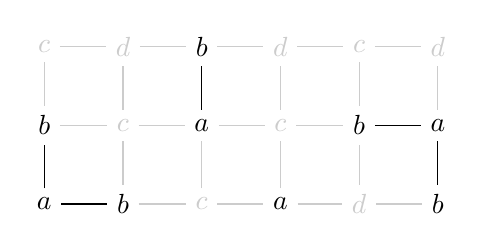
\begin{tikzpicture}[scale=1]
            \node (x11) at (0, 0) { $a$ };
            \node (x12) at (1, 0) { $b$ };
            \node[opacity=0.2] (x13) at (2, 0) { $c$ };
            \node (x21) at (0, 1) { $b$ };
            \node[opacity=0.2] (x22) at (1, 1) { $c$ };
            \node (x23) at (2, 1) { $a$ };
            \node[opacity=0.2] (x31) at (0, 2) { $c$ };
            \node[opacity=0.2] (x32) at (1, 2) { $d$ };
            \node (x33) at (2, 2) { $b$ };
            \node (y11) at (3, 0) { $a$ };
            \node[opacity=0.2] (y12) at (4, 0) { $d$ };
            \node (y13) at (5, 0) { $b$ };
            \node[opacity=0.2] (y21) at (3, 1) { $c$ };
            \node (y22) at (4, 1) { $b$ };
            \node (y23) at (5, 1) { $a$ };
            \node[opacity=0.2] (y31) at (3, 2) { $d$ };
            \node[opacity=0.2] (y32) at (4, 2) { $c$ };
            \node[opacity=0.2] (y33) at (5, 2) { $d$ };
    
            \draw (x11) -- (x12);
            \draw[opacity=0.2] (x12) -- (x13);
    
            \draw[opacity=0.2] (x21) -- (x22);
            \draw[opacity=0.2] (x22) -- (x23);
            \draw[opacity=0.2] (x31) -- (x32);
            \draw[opacity=0.2] (x32) -- (x33);
    
            \draw (x11) -- (x21);
            \draw[opacity=0.2] (x21) -- (x31);
            \draw[opacity=0.2] (x12) -- (x22) -- (x32);
            \draw[opacity=0.2] (x13) -- (x23);
            \draw (x23) -- (x33);
    
            \draw[opacity=0.2] (y11) -- (y12) -- (y13);
            \draw[opacity=0.2] (y21) -- (y22);
            \draw (y22) -- (y23);
            \draw[opacity=0.2] (y31) -- (y32) -- (y33);
    
            \draw[opacity=0.2] (y11) -- (y21) -- (y31);
            \draw[opacity=0.2] (y12) -- (y22) -- (y32);
            \draw (y13) -- (y23);
            \draw[opacity=0.2] (y23) -- (y33);
    
            \draw[opacity=0.2] (x13) -- (y11);
            \draw[opacity=0.2] (x23) -- (y21);
            \draw[opacity=0.2] (x33) -- (y31);
        \end{tikzpicture}
        \caption{We write $\chain{v_1}{v_2}{ab}$ to indicate $v_1$ and $v_2$ lie on the same $ab$-chain.}
    \end{figure}
    
\end{frame}

\begin{frame}
    \frametitle{Ring schemes}

    \begin{definition}
        Given a coloring $x$ of a planar graph $G$ and the colors on its ring $x(R)$. The \emph{scheme} on $R$ of $x$ consists of $x(R)$ with knowledge whether $u \in \kappa_{ab}(v)$ for two ring vertices $u,v \in R$ and colors $ab$.
    \end{definition}
    \begin{figure}[!ht]
        \centering
        \begin{tikzpicture}[scale=1.0, mid arrow/.style={
            postaction={ decorate, decoration={ markings, mark=at position 0.6 with { \arrow[black]{>>} } } } }]
    
            \node[circle, fill, scale=0.015cm, opacity=0.2] (v) at (0, 0) { };
            \node[circle, fill, scale=0.015cm, label=above:$a$] (l1) at (0, 1) { };
            \node[circle, fill, scale=0.015cm, label=right:$b$] (l2) at (0.9, 0.30) { };
            \node[circle, fill, scale=0.015cm, label=below:$c$] (l3) at (0.6, -0.77) {};
            \node[circle, fill, scale=0.015cm, label=below:$a$] (l4) at (-0.6, -0.77) {};
            \node[circle, fill, scale=0.015cm, label=left:$b$] (l5) at (-0.9, 0.30) {};
            \node[circle, fill, scale=0.015cm, label=above:$c$] (c1) at (0.7, 1) {};
            \node[circle, fill, scale=0.015cm, label=right:$a$] (c2) at (1.32, 0.68) {};
            \node[circle, fill, scale=0.015cm, label=right:$c$] (c3) at (1.45, 0.05) {};
            \node[circle, fill, scale=0.015cm, label=right:$a$] (c4) at (1.1, -0.49) {};
            \draw[mid arrow] (l1) -- (l2);
            \draw (l2) -- (l3) -- (l4) -- (l5) -- (l1);
            \draw (l1) -- (c1) -- (c2) -- (c3) -- (c4) -- (l3);
            \draw[opacity=0.2] (l1) -- (v);
            \draw[opacity=0.2] (l2) -- (v);
            \draw[opacity=0.2] (l3) -- (v);
            \draw[opacity=0.2] (l4) -- (v); 
            \draw[opacity=0.2] (l5) -- (v);
            \node (impl) at (3, 0) { $\hspace{1cm} \implies \hspace{0.3cm} \begin{matrix}
                \scheme{a,b,c,a,b}{ 13a } \\
                \scheme{a,b,c,a,b}{ 25d- }
            \end{matrix}$ };
        \end{tikzpicture}
    \caption{The edge with $\gg$ indicates order of vertices in the coloring.}
    \end{figure}
\end{frame}

\begin{frame}
    \frametitle{Schemes imply new colorings}
    \begin{definition}
        Given two schemes $x$ and $y$. We say that $x$ implies $y$ if $x=y$ or $y$ can be obtained from $x$ by flipping a Kempe-chain. Write $x\compat y$.
    \end{definition}
    
    \begin{equation*}
        \scheme{a,b,c,a,b}{ 13a } \compat \scheme{a,b,c,a,\textbf{d}}{{13a}}, \quad \quad
        \scheme{a,b,c,a,b}{ 25d- } \compat \scheme{a,\textbf{d},c,a,b}{{25d-}}.
    \end{equation*}

    \vspace{1cm}
    This is the key argument we used in the five color theorem!
\end{frame}